\documentclass[aspectratio=169,11pt]{beamer}

\usetheme{Madrid}
\usecolortheme{default}
\usepackage{booktabs}
\usepackage{amsmath}
\usepackage{graphicx}
\usepackage{xcolor}
\usepackage{tikz}
\usetikzlibrary{arrows.meta,positioning}

% ---------------- Style ----------------
\definecolor{ntuBlue}{RGB}{0,70,140}
\definecolor{softBlue}{RGB}{232,241,250}
\definecolor{darkGray}{RGB}{55,55,55}
\definecolor{goodGreen}{RGB}{32,130,80}
\definecolor{warnOrange}{RGB}{210,115,30}
\setbeamercolor{structure}{fg=ntuBlue}
\setbeamercolor{frametitle}{fg=white,bg=ntuBlue}
\setbeamertemplate{navigation symbols}{}
\setbeamertemplate{footline}[frame number]
\setbeamertemplate{itemize item}{\small$\blacktriangleright$}
\setbeamertemplate{itemize subitem}{\scriptsize--}
\setbeamersize{text margin left=0.8cm,text margin right=0.8cm}
\setbeamerfont{frametitle}{size=\Large}
\setbeamerfont{itemize/enumerate body}{size=\normalsize}
\setbeamerfont{itemize/enumerate subbody}{size=\small}

\newcommand{\code}[1]{\texttt{#1}}
\newcommand{\green}[1]{\textcolor{goodGreen}{#1}}
\newcommand{\orange}[1]{\textcolor{warnOrange}{#1}}
\newcommand{\imgbox}[2][0.30\textheight]{%
\begin{center}
\fbox{%
\begin{minipage}[c][#1][c]{0.88\textwidth}
\centering
\normalsize #2
\end{minipage}}
\end{center}}
\newcommand{\smallimgbox}[2][0.27\textheight]{%
\begin{center}
\fbox{%
\begin{minipage}[c][#1][c]{0.96\linewidth}
\centering
\scriptsize #2
\end{minipage}}
\end{center}}

\title[Stereo Matching]{Stereo Matching and 3D Reconstruction}
\subtitle{NTU Computer Vision Final Project -- Team 10}
\author{Team 10}
\institute{National Taiwan University}
\date{Spring 2026}

\begin{document}

% 中文逐字稿：
% 大家好，我們是第十組。我們實作了stereo matching的基礎部分和 bonus的3D reconstruction。接下來講我們程式實際是怎麼做的。
\begin{frame}
\titlepage
\end{frame}

% 中文逐字稿：
% 這是我們的大綱，會先快速介紹 basic 和 bonus 的實作流程，接著講 computeDisp 的設計，再看 basic 的結果和時間分析。後半部會說明 bonus的部分如何從 disparity 做到 mesh，最後播放我們的 demo 影片。
\begin{frame}{Outline}
\Large
\begin{itemize}
    \item Basic + bonus summary
    \item Basic implementation: \code{computeDisp.py}
    \item Basic results + runtime analysis
    \item Bonus implementation: disparity $\rightarrow$ depth $\rightarrow$ TSDF mesh
    \item Bonus demo: first-person walkthrough
\end{itemize}
\end{frame}

% 中文逐字稿：
% 我們的在computeDisp裡實作的stereo matching可以大致切分成以下流程：Census 建 cost、Weighted Guided Image Filter 做 cost aggregation、Winner-Takes-All 選 disparity，最後做Left-right consistency check、hole filling 和 weighted median。Bonus 則是重複使用這個 disparity，轉成 depth，丟進 Open3D的TSDF 做多視角融合，再輸出 mesh 和第一人稱走訪影片。
\begin{frame}{Quick summary}
\begin{center}
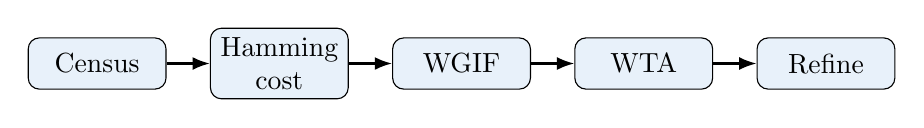
\begin{tikzpicture}[
  node distance=0.55cm,
  block/.style={draw, rounded corners, minimum height=0.65cm, minimum width=1.75cm, align=center, fill=softBlue},
  arrow/.style={-{Latex[length=2.2mm]}, thick}
]
  \node[block] (census) {Census};
  \node[block, right=of census] (ham) {Hamming\\cost};
  \node[block, right=of ham] (wgif) {WGIF};
  \node[block, right=of wgif] (wta) {WTA};
  \node[block, right=of wta] (refine) {Refine};
  \draw[arrow] (census) -- (ham);
  \draw[arrow] (ham) -- (wgif);
  \draw[arrow] (wgif) -- (wta);
  \draw[arrow] (wta) -- (refine);
\end{tikzpicture}
\end{center}

\vspace{0.35em}
\begin{itemize}
    \item \textbf{Basic:} classical stereo matcher in \code{computeDisp.py}
    \item \textbf{Bonus:} use predicted disparity for TartanAir 3D reconstruction
    \item \textbf{Output:} disparity maps, mesh, walkthrough video
\end{itemize}

\end{frame}

% 中文逐字稿：
% 這是 basic部分，computeDisp 的整體 pseudocode，先把輸入圖片轉成灰階，接著進入剛才介紹的pipeline，最後得到left disparity map。
\begin{frame}[fragile]{Basic: actual code path}
\begin{columns}[T,totalwidth=\textwidth]
\begin{column}{0.46\textwidth}
\begin{itemize}
    \item Start from grayscale for Census
    \item Build \textbf{left} cost volume
    \item Get \textbf{right} cost by reindexing
    \item Aggregate left cost only
    \item Final output: left disparity map
\end{itemize}
\end{column}
\begin{column}{0.50\textwidth}
\scriptsize
\begin{verbatim}
computeDisp(Il, Ir, max_disp):
  gray_L = BGR2GRAY(Il)
  gray_R = BGR2GRAY(Ir)

  cL = census_transform(gray_L)
  cR = census_transform(gray_R)

  cost_L = hamming_cost_volume(cL, cR)
  cost_R = reindex_cost_to_right(cost_L)

  cost_L = aggregate(cost_L, Il)

  D_L = argmin(cost_L, axis=d)
  D_R = argmin(cost_R, axis=d)

  labels = refine(D_L, D_R, cost_L, Il)
  return uint8(labels)
\end{verbatim}
\end{column}
\end{columns}
\end{frame}

% 中文逐字稿：
% 第一個實作環節是 Census transform。對每個 pixel，我們拿一個 9 乘 7 的 local window，然後把 window 裡的每個鄰居跟中心 pixel 比較。如果鄰居比中心點暗，就記成 1，否則記成 0。這樣每個 pixel 就不再只是一個灰階值，而是被轉成一串 binary pattern，描述它附近的亮暗結構。

% Census 的好處是，它比較的是「相對亮暗關係」，不是直接比較 intensity 數值。舉例來說，如果整張圖變亮一點，RGB 或灰階值可能會全部改變，但很多鄰居和中心點之間的大小關係仍然差不多。所以 Census 對亮度變化比較不敏感，也比較適合拿來做左右影像的 matching。
\begin{frame}[fragile]{Step 1: Census transform}
\begin{columns}[T,totalwidth=\textwidth]
\begin{column}{0.46\textwidth}
\begin{itemize}
    \item Window: \textbf{$9\times7$}
    \item $9\times7-1=62$ comparisons
    \item Stored in one \code{uint64}
    \item Border: replicated padding
    \item More stable than raw intensity difference
\end{itemize}
\vspace{0.3em}
\[
\text{bit}_i=[I(\text{neighbor}_i)<I(\text{center})]
\]
\end{column}
\begin{column}{0.50\textwidth}
\scriptsize
\begin{verbatim}
census_transform(gray):
  pad image by edge values
  code = zeros(H, W, uint64)

  for each offset in 9x7 window:
    if offset is center: continue
    bit = (neighbor < center)
    code |= bit << bit_index

  return code
\end{verbatim}
\end{column}
\end{columns}
\end{frame}

% 中文逐字稿：
% 這一步是建立 cost volume。我們先把每個 pixel 做 Census transform，也就是把周圍像素和中心點的亮暗關係存成 binary code。這樣比直接比較 RGB 更不容易受亮度變化影響。

% 接著對每個 disparity d，比較左圖 x 和右圖 x-d 的 Census code。比較方式是 XOR 加 popcount：不一樣的 bit 越少，Hamming cost 越低，代表兩個 patch 越相似。

% 最後把所有 disparity 的 cost map 疊起來，得到 shape 是 (max_disp+1, H, W) 的 cost volume。右圖方向的 cost volume 則用 reindexing 從左圖 cost volume 得到，避免重算一次。
\begin{frame}[fragile]{Step 1: Hamming cost volume}
\begin{columns}[T,totalwidth=\textwidth]
\begin{column}{0.46\textwidth}
\begin{itemize}
    \item Cost = bit differences
    \item Shape: $(D+1)\times H\times W$
    \item OOB columns: clamp to border
    \item Popcount path:
    \begin{itemize}
        \item \code{np.bitwise\_count}, if available
        \item SWAR fallback, otherwise
    \end{itemize}
    \item Parallel over disparity slices
\end{itemize}
\vspace{-0.2em}
\[
C(d,y,x)=\operatorname{popcount}(c_L(y,x)\oplus c_R(y,x-d))
\]
\end{column}
\begin{column}{0.50\textwidth}
\scriptsize
\begin{verbatim}
hamming_cost_volume(cL, cR):
  for d = 0 ... max_disp parallel:
    xR = clip(x - d, 0, W-1)
    xor = cL[y, x] XOR cR[y, xR]
    cost[d, y, x] = popcount(xor)

  return cost  # (D+1, H, W)
\end{verbatim}
\end{column}
\end{columns}
\end{frame}

% 中文逐字稿：
% 這裡是我們做的一個效率優化。後面的 Left-Right Consistency 需要同時有左圖 disparity 和右圖 disparity，所以理論上也要建立右圖視角的 cost volume。但如果直接重算一次，就等於 Hamming cost computation 要跑兩遍。

% 我們的做法是只真正計算左圖視角的 cost volume。因為 Hamming distance 是對稱的，也就是左邊 code 跟右邊 code 比，和右邊 code 跟左邊 code 比，結果是一樣的。差別只是在於對應的 x 座標要換一下。

% 所以對右圖某個位置 x' 來說，它對應到左圖的位置會是 x' + d。程式就利用這個關係，把左圖 cost volume 的 column 重新 indexing，直接得到右圖方向的 cost volume。這樣可以省掉一次完整的 Hamming cost 建立，速度會比較快。
\begin{frame}[fragile]{Optimization: right cost by reindexing}
\begin{columns}[T,totalwidth=\textwidth]
\begin{column}{0.46\textwidth}
\begin{itemize}
    \item Need \code{D\_R} only for LRC mask
    \item Hamming: symmetric matching cost
    \item Avoids another Hamming pass
    \item \code{cost\_R} stays \textbf{raw}, not WGIF-filtered
\end{itemize}
\vspace{0.3em}
\[
C_R(d,y,x_R)=C_L(d,y,\operatorname{clip}(x_R+d))
\]
\end{column}
\begin{column}{0.50\textwidth}
\scriptsize
\begin{verbatim}
reindex_cost_to_right(cost_L):
  for each disparity d:
    for each right column xR:
      xL = clip(xR + d, 0, W-1)
      cost_R[d, y, xR] = cost_L[d, y, xL]

  return cost_R
\end{verbatim}
\end{column}
\end{columns}
\end{frame}

% 中文逐字稿：
% 第二步是 cost aggregation。前面算出的 raw cost volume 只看很局部的 Census matching，所以會有很多雜訊。因此我們對每個 disparity slice 做 weight guided filtering，讓 cost map 變得比較平滑。

% 這裡的一個重點是我們不是單純用 box filter 平均，因為那樣會把物體邊界也一起模糊掉。我們使用左圖當作 guide image，讓 cost 在顏色或亮度相近的區域內被平滑，但在影像邊緣附近盡量保留變化。這樣可以減少錯誤 matching，同時不要把前景和背景的 disparity 混在一起。

% 右邊 pseudocode 是我們的 aggregate function。它先計算 guide image 的 mean 和 variance，接著對每一層 disparity cost slice 計算 guided filter 的線性係數 a 和 b，最後輸出平滑後的 cost volume。後面的 Winner Takes All 就會在這個比較穩定的 cost volume 上選最小 cost。
\begin{frame}[fragile]{Step 2: WGIF aggregation}
\begin{columns}[T,totalwidth=\textwidth]
\begin{column}{0.44\textwidth}
\begin{itemize}
    \item Guide: left image grayscale
    \item Filter each disparity cost slice
    \item Adaptive $\epsilon$ through \code{gamma}
    \item Edges: preserve discontinuities
    \item Flat regions: smooth stronger
    \item Parallel over slices again
\end{itemize}
\vspace{0.2em}
\[
q(x)=\bar a(x)I(x)+\bar b(x)
\]
\end{column}
\begin{column}{0.52\textwidth}
\scriptsize
\begin{verbatim}
aggregate(cost, guide):
  I = grayscale(guide) / 255
  mean_I = boxFilter(I)
  var_I  = boxFilter(I*I) - mean_I^2

  gamma = (var_I + eps0) / mean(var_I + eps0)
  denom = var_I + eps / gamma

  for each disparity slice p parallel:
    mean_p  = boxFilter(p)
    cov_Ip  = boxFilter(I*p) - mean_I*mean_p
    a = cov_Ip / denom
    b = mean_p - a*mean_I
    q = boxFilter(a)*I + boxFilter(b)
\end{verbatim}
\end{column}
\end{columns}
\end{frame}

% 中文逐字稿：
% 第三步是 WTA，也就是 Winner-Take-All。對每個 pixel，我們沿著 disparity 軸去看所有候選 disparity 的 cost，然後選 cost 最小的那個 d，作為這個 pixel 的 disparity。

% 在我們的實作裡，左圖 disparity 是用前面 WGIF 平滑後的 cost volume 算出來的，因為左圖 disparity 是最後要輸出的結果，所以希望它比較穩定、雜訊比較少。右圖 disparity 則是用剛剛 re-index 出來的 raw cost volume 直接做 WTA。

% 這樣做的原因是，右圖 disparity 不會作為最後輸出，它只會在下一步 Left-Right Consistency 裡，用來檢查左圖的 matching 是否合理。因此我們選擇不再對右圖 cost volume 做一次 guided filtering，這樣可以省下不少時間，而且對最後輸出的影響不大。
\begin{frame}[fragile]{Step 3: WTA selection}
\begin{columns}[T,totalwidth=\textwidth]
\begin{column}{0.48\textwidth}
\begin{itemize}
    \item One disparity per pixel
    \item \code{D\_L}: final candidate disparity
    \item \code{D\_R}: consistency helper
    \item Skips right-side aggregation
\end{itemize}
\vspace{0.3em}
\[
D_L(y,x)=\arg\min_d C_L(d,y,x)
\]
\end{column}
\begin{column}{0.48\textwidth}
\scriptsize
\begin{verbatim}
winner_take_all(cost):
  return argmin(cost, axis=disparity)

D_L = WTA(filtered cost_L)
D_R = WTA(raw cost_R)
\end{verbatim}
\end{column}
\end{columns}
\end{frame}


% 中文逐字稿：
% 最後一步是 refinement。程式先做 Left-Right Consistency，檢查左圖 disparity 對到右圖後，兩邊 disparity 是否差在 1 pixel 以內。不一致或超出邊界的點會被標成 invalid。

% 接著 hole filling 是逐列做左右 sweep。從左掃一次、從右掃一次，各自記住最近的有效 disparity，最後每個 invalid pixel 取兩邊較小的值。邊界初始值設成 max_disp，避免整列前後都是 hole 時被錯誤填成 0。

\begin{frame}[fragile]{Step 4: Refinement: LRC + hole filling}
\begin{columns}[T,totalwidth=\textwidth]
\begin{column}{0.44\textwidth}
\begin{itemize}
    \item Check left/right agreement
    \item Invalid if:
    \begin{itemize}
        \item matched $x$ out of bound
        \item disparity difference $>1$
    \end{itemize}
    \item Fill holes row by row
    \item Use nearest valid from left/right
    \item Final fill = smaller one
\end{itemize}
\[
|D_L(y,x)-D_R(y,x-D_L(y,x))|\le 1
\]
\end{column}

\begin{column}{0.52\textwidth}
\scriptsize
\begin{verbatim}
valid = LR_consistency(D_L, D_R)

for each row:
  left_fill  = sweep_left_to_right()
  right_fill = sweep_right_to_left()

filled = min(left_fill, right_fill)
\end{verbatim}
\end{column}
\end{columns}
\end{frame}


% 中文逐字稿：
% 接著是 sub-pixel 和 weighted median。有效 pixel 會用 WTA 選到的整數 disparity d，再看 cost volume 裡 d-1、d、d+1 三個位置的 cost，fit 一個小 parabola，估計小數位移 delta。invalid pixel 則不用 sub-pixel，直接使用前面 hole filling 的結果。

% 最後進 weighted median filter，我們在這裡加了一個步驟，先做 BGR quantization，把每個 channel 從 256 levels 降到 16 levels。這樣可以降低細小顏色雜訊對 filter 的影響，同時大部分物體邊界仍然保留下來。

\begin{frame}[fragile]{Step 4: Refinement: sub-pixel + weighted median}
\begin{columns}[T,totalwidth=\textwidth]
\begin{column}{0.46\textwidth}
\begin{itemize}
    \item Valid pixels:
    \begin{itemize}
        \item refine integer $d$ by parabola fitting
        \item use cost at $d-1,d,d+1$
    \end{itemize}
    \item Invalid pixels:
    \begin{itemize}
        \item use hole-filled disparity
    \end{itemize}
    \item Then weighted median smoothing
    \item Guide image: quantized left BGR
    \item Final output is \code{uint8}
\end{itemize}
\end{column}

\begin{column}{0.51\textwidth}
\scriptsize
\begin{verbatim}
d_sub = subpixel_refine(D_L, cost_L)

d = where(valid, d_sub, filled_int)

disp_u8 = clip(d).astype(uint8)

guide_q = ((guide_bgr >> 4) << 4)

return weightedMedianFilter(
  joint=guide_q,
  src=disp_u8,
  r=15)
\end{verbatim}
\end{column}
\end{columns}
\end{frame}

% 中文逐字稿：
% 這裡是basic 在codelab 上 public set 取得的最好結果。Bad Pixel Rate的部分。Tsukuba 大約 3.4，Venus 0.31，Teddy 10.09。Venus 特別好是因為場景比較平滑、平面結構明顯；Teddy 因為 occlusion、細邊界和重複紋理，所以錯誤較高。
\begin{frame}{Basic results}
\begin{table}
\centering
\large
\begin{tabular}{lcc}
\toprule
Image & BPR & Time \\
\midrule
Tsukuba & 3.41\% & 0.177 s \\
Venus & 0.31\% & 0.196 s \\
Teddy & 10.09\% & 0.336 s \\
\bottomrule
\end{tabular}
\end{table}

\begin{itemize}
    \item Venus: clean plane structure $\rightarrow$ lowest BPR
    \item Tsukuba: moderate texture, stable result
    \item Teddy: occlusion + thin structure $\rightarrow$ harder
    \item Cones / hidden results: checked using TA score sheet
\end{itemize}
\end{frame}

% 中文逐字稿：
% 我們還觀察到一個現象，為什麼一樣的 code，在 CodaLab 上不同 submission 的時間會差很多？我們覺得這主要是因為我們程式時間跟 CPU thread scheduling 很有關。Cost volume 和 WGIF 都對 disparity slice 開 thread pool，而且 worker 數會根據 os.cpu_count 決定，上限是 8。如果 CodaLab 當時機器比較忙、cache 或 memory bandwidth 競爭比較強，時間就可能變慢，但 BPR 通常不會因此大幅改變。
\begin{frame}[fragile]{Why CodaLab runtime varies}
\begin{columns}[T,totalwidth=\textwidth]
\begin{column}{0.46\textwidth}
\begin{itemize}
    \item Same code, different grader load
    \item Thread scheduling affects wall time
    \item Cost volume is memory-bandwidth heavy
    \item Cache effects vary by machine
    \item BPR stable; runtime less stable
\end{itemize}
\end{column}
\begin{column}{0.50\textwidth}
\scriptsize
\begin{verbatim}
_MAX_WORKERS = min(os.cpu_count() or 4, 8)

parallel loops:
  1. hamming_cost_volume
  2. aggregate / WGIF

memory use:
  cost volume = (D+1, H, W) float32
\end{verbatim}
\end{column}
\end{columns}
\end{frame}

% 中文逐字稿
% 接下來是 bonus部分。我們的Bonus 是把每一張 stereo pair 的 disparity 轉成 depth，再用相機 pose 把多張 depth map 融合到同一個 TSDF volume。這裡我們選用 TartanAir 是因為它有 stereo、depth 和 pose，方便做重建和對照。
\begin{frame}{Bonus: pipeline overview}
\begin{center}
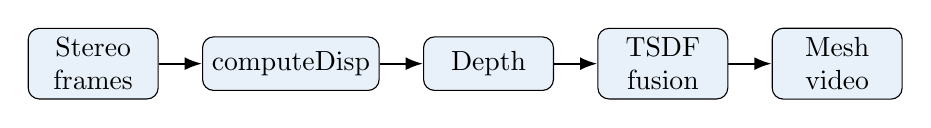
\begin{tikzpicture}[
  node distance=0.55cm,
  block/.style={draw, rounded corners, minimum height=0.68cm, minimum width=1.65cm, align=center, fill=softBlue},
  arrow/.style={-{Latex[length=2.2mm]}, thick}
]
  \node[block] (stereo) {Stereo\\frames};
  \node[block, right=of stereo] (disp) {computeDisp};
  \node[block, right=of disp] (depth) {Depth};
  \node[block, right=of depth] (tsdf) {TSDF\\fusion};
  \node[block, right=of tsdf] (mesh) {Mesh\\video};
  \draw[arrow] (stereo) -- (disp);
  \draw[arrow] (disp) -- (depth);
  \draw[arrow] (depth) -- (tsdf);
  \draw[arrow] (tsdf) -- (mesh);
\end{tikzpicture}
\end{center}

\begin{itemize}
    \item Dataset: TartanAir \code{japanesealley/Hard/P000}
    \item Reuse \code{computeDisp} output
    \item Fuse many frames instead of showing one noisy depth map
\end{itemize}
\end{frame}

% 中文逐字稿：
% 我們選 TartanAir 的 japanesealley Hard P000 軌跡前 100 frame 作為示範。
% 它同時提供 stereo 影像、ground truth depth 和相機 pose，這三樣東西讓我們可以一邊做 3D 重建一邊算 BPR 驗證。
% TartanAir V1 所有場景內參都統一 fx=fy=320, cx=320, cy=240, baseline 0.25 m，影像大小 640 乘 480。
% 一個重要的小細節是 TartanAir 把天空跟超出感測範圍的 depth 標成接近 float16 最大值，大約 65504，後面 mask invalid 會用到。
\begin{frame}[fragile]{Bonus: dataset layout}
\begin{columns}[T,totalwidth=\textwidth]
\begin{column}{0.46\textwidth}
\begin{itemize}
    \item Synthetic: stereo + GT depth + GT pose all in one
    \item Intrinsics constant across V1
    \begin{itemize}
        \item $f_x = f_y = 320$, $c_x = 320$, $c_y = 240$
        \item baseline \code{0.25}\,m, image \code{640x480}
    \end{itemize}
    \item Sky / inf marked $\approx$ \code{65504} (float16 max)
    \item Pose: NED body axes (will fix next slide)
\end{itemize}
\end{column}
\begin{column}{0.50\textwidth}
\scriptsize
\begin{verbatim}
data/.../japanesealley/Hard/P000/
  image_left/  000XXX_left.png
  image_right/ 000XXX_right.png
  depth_left/  000XXX_left_depth.npy
  pose_left.txt   # 7 cols per row:
                  # tx ty tz qx qy qz qw
\end{verbatim}
\end{column}
\end{columns}
\end{frame}

% 中文逐字稿：
% 這是 bonus pipeline 裡最關鍵的一個技術細節。
% TartanAir 的 pose 是用 NED 機體座標系存的，也就是 x 朝前、y 朝右、z 朝下。
% 但 Open3D 跟 OpenCV 預期的相機座標系是 x 朝右、y 朝下、z 朝前。
% 如果直接拿 pose 用，深度沿 z 朝前反投影，但 pose 卻把 z 解讀成往下，所有重建的點就會飄到原始軌跡上方好幾公尺，整個 mesh 像懸空。
% 修法是把每個 pose 右乘一個固定的 4 乘 4 axis permutation matrix。Sanity check 就是左右相機的 translation 差 0.25 公尺，剛好對到資料集的 baseline，驗證單位跟旋轉一致。
\begin{frame}[fragile]{Bonus: pose NED $\rightarrow$ OpenCV ($\star$ key fix)}
\begin{columns}[T,totalwidth=\textwidth]
\begin{column}{0.44\textwidth}
\begin{itemize}
    \item TartanAir: \textbf{NED body} axes
    \begin{itemize}
        \item $x$ forward, $y$ right, $z$ down
    \end{itemize}
    \item Open3D / OpenCV: \textbf{camera} axes
    \begin{itemize}
        \item $x$ right, $y$ down, $z$ forward
    \end{itemize}
    \item \orange{Skip $\rightarrow$ mesh floats 3--15\,m above path}
    \item Fix: right-multiply by fixed permutation
\end{itemize}
\[
T^{\text{CV}}_{wc} = T^{\text{NED}}_{wc} \cdot M_{\text{NED}\to\text{CV}}
\]
Sanity: $\|t_L - t_R\| = 0.2500$\,m
\end{column}
\begin{column}{0.52\textwidth}
\scriptsize
\[
M_{\text{NED}\to\text{CV}} =
\begin{pmatrix}
0 & 0 & 1 & 0 \\
1 & 0 & 0 & 0 \\
0 & 1 & 0 & 0 \\
0 & 0 & 0 & 1
\end{pmatrix}
\]
\begin{verbatim}
load_poses(traj_dir, indices):
  rows = loadtxt(pose_left.txt)
  for i in indices:
    R = quat_to_R(qx, qy, qz, qw)
    T = build_4x4(R, t)
    out.append(T @ M_NED2CV)
  return out
\end{verbatim}
\end{column}
\end{columns}
\end{frame}

% 中文逐字稿：
% 拿到 disparity 之後，用立體幾何公式 Z 等於 fx 乘 baseline 除以 d 直接換成 depth。
% 但有兩種 pixel 必須先標成無效再餵進 TSDF。
% 第一是天空，TartanAir 把這些 pixel 標成接近 float16 最大值，所以 depth 大於等於 65000 的點直接歸零。
% 第二是太遠的 pixel，因為 stereo depth uncertainty 隨距離平方成長，超過 depth_trunc 就大多是 noise。
% 為什麼一定要顯式歸零，這是因為 Open3D TSDF 對 depth 等於 0 會直接 skip，但對「超過 trunc 的值」會 clip 成 trunc 距離，等於在 15 公尺處長一片幻影牆，整個重建就壞掉。
\begin{frame}[fragile]{Bonus: disparity $\rightarrow$ depth + invalid mask}
\begin{columns}[T,totalwidth=\textwidth]
\begin{column}{0.46\textwidth}
\begin{itemize}
    \item Triangulation: $Z = f_x \cdot B / d$
    \item \textbf{Two invalid bands} must both be zeroed
    \begin{itemize}
        \item sky: \code{depth >= 65000}
        \item far: \code{depth > depth\_trunc}
    \end{itemize}
    \item Open3D treats \code{depth=0} as invalid (skip)
    \item Else: clips far points $\rightarrow$ \orange{phantom wall at 15\,m}
\end{itemize}
\end{column}
\begin{column}{0.50\textwidth}
\scriptsize
\begin{verbatim}
disparity_to_depth(disp, fx, B):
  mask = disp >= 1.0
  depth[mask] = fx * B / disp[mask]
  return depth  # float32 metres

prepare_depth(depth, depth_trunc):
  out = depth.copy()
  out[out >= SKY_THRESHOLD] = 0
  out[out > depth_trunc]    = 0
  return out
\end{verbatim}
\end{column}
\end{columns}
\end{frame}

% 中文逐字稿：
% TSDF 的部分我們用 Open3D 的 ScalableTSDFVolume，它是一個 sparse voxel hash，能放得下整條巷弄而不爆 memory。
% Voxel size 設 0.05 公尺也就是 5 公分，因為 TartanAir 的巷弄寬度大約 10 到 20 公尺，5 公分的解析度可以保留牆面細節，又不會 voxel 數爆掉。
% sdf_trunc 設成 voxel 的 4 倍，是業界常用比例。
% depth_trunc 15 公尺是因為 stereo depth uncertainty 隨距離平方成長，太遠的 sample 多半是 noise，留下來只會把 mesh 拉花。
\begin{frame}[fragile]{Bonus: TSDF parameter rationale}
\begin{columns}[T,totalwidth=\textwidth]
\begin{column}{0.44\textwidth}
\begin{itemize}
    \item \code{ScalableTSDFVolume}: sparse voxel hash, scales to outdoor scenes
    \item \code{voxel\_size = 0.05}\,m
    \begin{itemize}
        \item alley width $\sim$10--20\,m
        \item 5\,cm keeps walls sharp
    \end{itemize}
    \item \code{sdf\_trunc = 4 $\times$ voxel}
    \item \code{depth\_trunc = 15}\,m
    \begin{itemize}
        \item stereo noise $\propto Z^2 / (f_x B)$
    \end{itemize}
\end{itemize}
\end{column}
\begin{column}{0.52\textwidth}
\scriptsize
\begin{verbatim}
TSDFConfig:
  voxel_size  = 0.05   # metres
  sdf_trunc   = 0.20   # 4x voxel
  depth_trunc = 15.0   # metres
  depth_scale = 1000   # m -> uint16 mm

make_volume(cfg):
  return ScalableTSDFVolume(
    voxel_length=cfg.voxel_size,
    sdf_trunc=cfg.sdf_trunc,
    color_type=RGB8,
  )
\end{verbatim}
\end{column}
\end{columns}
\end{frame}

% 中文逐字稿：
% 對每一張 frame，我們把 RGB 圖跟 depth 包成 RGBDImage，配上相機內參跟 pose 的反矩陣丟進 TSDF integrate。
% 為什麼是 pose 的反矩陣，因為 Open3D 要的 extrinsic 是 camera 看 world 的方向，而我們手上的 pose 是 world 對 camera，要先反過來。
% TSDF 內部會根據視角加權，多個 frame 看到同一面牆的 sample 會互相強化，per-frame 的隨機 noise 會被平均掉。
% 這也是為什麼 v6 BPR 雖然 20 趴，但最後 mesh 看起來仍然連貫——multi-view fusion 把單張 noise 壓掉了。
\begin{frame}[fragile]{Bonus: per-frame integration}
\begin{columns}[T,totalwidth=\textwidth]
\begin{column}{0.44\textwidth}
\begin{itemize}
    \item Pack RGB + depth into \code{RGBDImage}
    \item depth (m) $\rightarrow$ \code{uint16} millimetres
    \item Open3D wants extrinsic $= T_{cam \leftarrow world}$
    \begin{itemize}
        \item invert our $T_{world \leftarrow cam}$
    \end{itemize}
    \item TSDF weights samples by viewing angle
    \item \green{Per-frame stereo noise cancels across views}
\end{itemize}
\end{column}
\begin{column}{0.52\textwidth}
\scriptsize
\begin{verbatim}
integrate_frame(vol, Il, depth,
                K, T_world_cam, cfg):
  rgb = BGR2RGB(Il)
  depth_clip = clip(depth, 0, trunc)
  depth_mm   = (depth_clip * 1000).uint16
  rgbd = RGBDImage(rgb, depth_mm)

  K_o3d = PinholeCameraIntrinsic(
            W, H, fx, fy, cx, cy)
  extr  = inv(T_world_cam)
  vol.integrate(rgbd, K_o3d, extr)
\end{verbatim}
\end{column}
\end{columns}
\end{frame}

% 中文逐字稿：
% 100 個 frame 都 integrate 完之後，從 TSDF 抽出 triangle mesh，這是 sparse marching cubes，Open3D 內建。
% 影片渲染我們刻意選 follow-trajectory，也就是把虛擬相機放回每個原始拍攝姿態上，而不是用 orbit 環繞。
% 這樣做有兩個好處。第一是不用煩惱合成資料集 world frame 的 up 軸到底朝哪邊，pose 本身就告訴我們相機的 up。
% 第二是出來的影片可以跟原始 left image 像素級重疊，只要對得起來就是重建品質的直接視覺證據，比 orbit 更有說服力。
% 渲染用 Open3D OffscreenRenderer，走 EGL headless，不需要 X server。畫面 2 倍 upscale，內參同步放大，保持 aspect ratio。
\begin{frame}[fragile]{Bonus: mesh extract + first-person render}
\begin{columns}[T,totalwidth=\textwidth]
\begin{column}{0.46\textwidth}
\begin{itemize}
    \item Sparse marching cubes from TSDF
    \item \textbf{Follow-trajectory}, not orbit
    \begin{itemize}
        \item virtual cam at each capture pose
        \item video overlaps original frames
        \item sidesteps world-up ambiguity
    \end{itemize}
    \item \code{OffscreenRenderer}: EGL headless
    \item Render $2\times$ upscale, $K$ scaled to match
\end{itemize}
\end{column}
\begin{column}{0.50\textwidth}
\scriptsize
\begin{verbatim}
mesh = vol.extract_triangle_mesh()
mesh.compute_vertex_normals()

render_follow_trajectory(mesh, poses,
                         K, (W, H)):
  renderer = OffscreenRenderer(rW, rH)
  scene.add_geometry(mesh, defaultLit)
  for T_world_cam in poses:
    T_cam_world = inv(T_world_cam)
    renderer.setup_camera(K_up, T_cam_world)
    frames.append(renderer.render_to_image())
  write_mp4(frames, fps=15, codec=libx264)
\end{verbatim}
\end{column}
\end{columns}
\end{frame}

% 中文逐字稿：
% 量化結果這邊，我們用 GT depth 換算成 GT disparity 跟我們的預測比較，valid mask 排除天空跟超出搜尋範圍的 pixel。
% v6 在 1 px 的 BPR 平均 20.21%，3 px 是 10.75%。這個數字在 TartanAir 合成資料集上的古典 stereo 是合理水準。
% 我們也試了 v8，加了 sub-pixel refinement，但 BPR 跟 v6 幾乎打平。原因是 computeDisp 介面回傳 uint8，sub-pixel 的小數部分在這個 API 邊界就被 clip 掉了。
% 最後我們把 NVIDIA CVPR 2025 Best Paper Nomination 的 FoundationStereo 接進來，BPR 從 20% 直接掉到 3.65%，最佳 frame 0.74%，3 px 中位數已經破 1%。這顯示古典方法在合成資料集上的確有結構性限制，要靠 deep prior 才能真正突破。
\begin{frame}{Bonus: BPR vs TartanAir GT depth}
\begin{table}
\centering
\large
\begin{tabular}{lccc}
\toprule
Matcher & BPR @ 1\,px & BPR @ 3\,px & time / frame \\
\midrule
v6 (classical)               & 20.21\% & 10.75\% & 0.36\,s \\
v8 (classical + sub-pixel)   & 20.26\% & 10.75\% & 0.34\,s \\
\textbf{FoundationStereo}    & \green{\textbf{3.65\%}}  & \green{\textbf{1.23\%}}  & 0.28\,s \\
\bottomrule
\end{tabular}
\end{table}

\vspace{0.4em}
\begin{itemize}
    \item Setup: \code{japanesealley/Hard/P000} frames 0--99, \code{max\_disp=64}
    \item Classical hits the texture-poor ceiling at $\sim$20\%
    \item v8 sub-pixel gains lost at \code{uint8} API boundary
    \item Deep model (zero-shot): median BPR \green{0.91\%} @ 3\,px
\end{itemize}
\end{frame}

% 中文逐字稿：
% 最後是我們的 demo 影片。同一條 100 frame 的軌跡，同一條 TSDF pipeline，只有 matcher 換掉。
% 第一支是 v6 古典版本，第二支是 FoundationStereo zero-shot 深度版本，第三支是用 GT depth 做的 upper bound 參考。
% 看影片就能直接比較三者的牆面跟地面品質，不需要再看數字。
\begin{frame}{Bonus: demo videos}
\begin{center}
\begin{tabular}{ll}
\toprule
Version & File \\
\midrule
v6 (classical baseline)        & \code{out/v6\_demo.mp4} \\
FoundationStereo (deep)        & \code{out/foundation\_stereo\_demo.mp4} \\
GT depth (upper bound)         & \code{out/tartanair\_p000\_gt\_100.mp4} \\
\bottomrule
\end{tabular}
\end{center}

\vspace{0.6em}
\begin{itemize}
    \item Same 100-frame TartanAir trajectory
    \item Same TSDF pipeline; only the matcher changes
    \item Visual: cleaner walls and ground plane on the deep version
\end{itemize}
\end{frame}

\end{document}
